%%%%%%%%%%%%%%%%%%%%%%%%%%%%%%%%%%%%%%%%%
% Arsclassica Article
% LaTeX Template
% Version 1.1 (10/6/14)
%
% This template has been downloaded from:
% http://www.LaTeXTemplates.com
%
% Original author:
% Lorenzo Pantieri (http://www.lorenzopantieri.net) with extensive modifications by:
% Vel (vel@latextemplates.com)
%
% License:
% CC BY-NC-SA 3.0 (http://creativecommons.org/licenses/by-nc-sa/3.0/)
%
%%%%%%%%%%%%%%%%%%%%%%%%%%%%%%%%%%%%%%%%%

%----------------------------------------------------------------------------------------
%	PACKAGES AND OTHER DOCUMENT CONFIGURATIONS
%----------------------------------------------------------------------------------------

\documentclass[
10pt, % Main document font size
a4paper, % Paper type, use 'letterpaper' for US Letter paper
oneside, % One page layout (no page indentation)
%twoside, % Two page layout (page indentation for binding and different headers)
headinclude,footinclude, % Extra spacing for the header and footer
BCOR5mm, % Binding correction
]{scrartcl}

%%%%%%%%%%%%%%%%%%%%%%%%%%%%%%%%%%%%%%%%%
% Arsclassica Article
% Structure Specification File
%
% This file has been downloaded from:
% http://www.LaTeXTemplates.com
%
% Original author:
% Lorenzo Pantieri (http://www.lorenzopantieri.net) with extensive modifications by:
% Vel (vel@latextemplates.com)
%
% License:
% CC BY-NC-SA 3.0 (http://creativecommons.org/licenses/by-nc-sa/3.0/)
%
%%%%%%%%%%%%%%%%%%%%%%%%%%%%%%%%%%%%%%%%%

%----------------------------------------------------------------------------------------
%	REQUIRED PACKAGES
%----------------------------------------------------------------------------------------

\usepackage[
nochapters, % Turn off chapters since this is an article        
beramono, % Use the Bera Mono font for monospaced text (\texttt)
pdfspacing, % Makes use of pdftex’ letter spacing capabilities via the microtype package
dottedtoc % Dotted lines leading to the page numbers in the table of contents
]{classicthesis} % The layout is based on the Classic Thesis style


\usepackage[T1]{fontenc} % Use 8-bit encoding that has 256 glyphs

\usepackage[utf8]{inputenc} % Required for including letters with accents

\usepackage{graphicx} % Required for including images
\graphicspath{{Figures/}} % Set the default folder for images

\usepackage{enumitem} % Required for manipulating the whitespace between and within lists

\usepackage{lipsum} % Used for inserting dummy 'Lorem ipsum' text into the template

\usepackage{subfig} % Required for creating figures with multiple parts (subfigures)

\usepackage{amsmath,amssymb,amsthm} % For including math equations, theorems, symbols, etc

\usepackage{varioref} % More descriptive referencing

\usepackage{hyperref}

%----------------------------------------------------------------------------------------
%	THEOREM STYLES
%---------------------------------------------------------------------------------------

\theoremstyle{definition} % Define theorem styles here based on the definition style (used for definitions and examples)
\newtheorem{definition}{Definition}

\theoremstyle{plain} % Define theorem styles here based on the plain style (used for theorems, lemmas, propositions)
\newtheorem{theorem}{Theorem}

\theoremstyle{remark} % Define theorem styles here based on the remark style (used for remarks and notes)

%----------------------------------------------------------------------------------------
%	HYPERLINKS
%---------------------------------------------------------------------------------------

\hypersetup{
%draft, % Uncomment to remove all links (useful for printing in black and white)
colorlinks=true, breaklinks=true, bookmarks=true,bookmarksnumbered,
urlcolor=webbrown, linkcolor=RoyalBlue, citecolor=webgreen, % Link colors
pdftitle={}, % PDF title
pdfauthor={\textcopyright}, % PDF Author
pdfsubject={}, % PDF Subject
pdfkeywords={}, % PDF Keywords
pdfcreator={pdfLaTeX}, % PDF Creator
pdfproducer={LaTeX with hyperref and ClassicThesis} % PDF producer
} % Include the structure.tex file which specified the document structure and layout

\hyphenation{Fortran hy-phen-ation} % Specify custom hyphenation points in words with dashes where you would like hyphenation to occur, or alternatively, don't put any dashes in a word to stop hyphenation altogether

%----------------------------------------------------------------------------------------
%	TITLE AND AUTHOR(S)
%----------------------------------------------------------------------------------------

\title{\normalfont\spacedallcaps{Model of Car}} % The article title

\author{\spacedlowsmallcaps{Johannes Milz}} % The article author(s) - author affiliations need to be specified in the AUTHOR AFFILIATIONS block

\date{} % An optional date to appear under the author(s)

%----------------------------------------------------------------------------------------
\usepackage{graphicx}

\begin{document}

%----------------------------------------------------------------------------------------
%	HEADERS
%----------------------------------------------------------------------------------------

\renewcommand{\sectionmark}[1]{\markright{\spacedlowsmallcaps{#1}}} % The header for all pages (oneside) or for even pages (twoside)
%\renewcommand{\subsectionmark}[1]{\markright{\thesubsection~#1}} % Uncomment when using the twoside option - this modifies the header on odd pages
\lehead{\mbox{\llap{\small\thepage\kern1em\color{halfgray} \vline}\color{halfgray}\hspace{0.5em}\rightmark\hfil}} % The header style

\pagestyle{scrheadings} % Enable the headers specified in this block

%----------------------------------------------------------------------------------------
%	TABLE OF CONTENTS & LISTS OF FIGURES AND TABLES
%----------------------------------------------------------------------------------------

\maketitle % Print the title/author/date block

\setcounter{tocdepth}{2} % Set the depth of the table of contents to show sections and subsections only

\tableofcontents % Print the table of contents

\section*{Notation}

\begin{tabular}{ |l | c | r }
  \hline                       
$\beta$  & steering angle \\
$\mu(s) = \sum_{k=0}^2 \bar{\mu}_k s^k$ & \href{http://www.wolframalpha.com/input/?i=interpolate+polynom+&f1={{1%2C+0.9}%2C{0.5%2C0.7}%2C{0%2C0.1}}&f=InterpolatingPolynomialCalculator.data2_{{1%2C+0.9}%2C{0.5%2C0.7}%2C{0%2C0.1}}&a=*FVarOpt.1-_***InterpolatingPolynomialCalculator.data2--.***InterpolatingPolynomialCalculator.data---.*--}{static friction} \\
$r$ & osculating circle \\
$\omega$ & velocity of steering angel\\
$w$ & weather\\

  \hline  
\end{tabular}



\section{ODE}
If the maximum static friction $\mu(w(t)) m g$ is greater than or equal $\sqrt{\left(\frac{mv(t)^2}{r(t)}\right)^2+ \left(m \dot{v}\right)^2},$ the car does not slide. The dynamics reads as
\begin{align*}
 &\dot{y} = v(t) \cos\beta(t)\\
& \dot{z} = v(t) \sin\beta(t) \\
& \dot{v} = \frac{1}{m}\left( \frac{M(t)}{R} - F_B(t) - \frac{1}{2}  c_w  \rho  A v(t)^2 - \left(f_{R0} + f_{R1} v(t) + f_{R4}v(t)^4 \right) m g\right)\\
& \dot{\beta} = \omega_{\beta} 
\end{align*}
If the maximum static friction is less than $F_{res}(t) = \sqrt{\left(\frac{mv(t)^2}{r(t)}\right)^2+ \left(m \dot{v}\right)^2},$ the car slides. The rolling friction $\left(f_{R0} + f_{R1} v(t) + f_{R4}v(t)^4 \right) m g$ "turns into" dynamic friction $\mu_d m g.$ For simplicity, we could assume that the coefficient $\mu_d$ is constant. However, $\mu_d \approx 0.5 \cdot \mu(w(t)),$ in general.
The dynamics reads as
\begin{align*}
 &\dot{y} = v(t) \cos\beta(t) +  v_r(t)\sin ( \frac{\pi}{2}+\alpha(t) +\beta(t)) \\
& \dot{z} = v(t) \sin\beta(t) +  v_r(t)\cos ( \frac{\pi}{2}+\alpha(t) +\beta(t)) \\
& \dot{v} = \frac{1}{m}\left( \frac{M(t)}{R} - F_B(t) - \frac{1}{2}  c_w  \rho  A v(t)^2 - \mu_d m g\right)\\
& \dot{\beta} = \omega_{\beta},
\end{align*}
where $\tan \alpha(t) = \frac{v(t)^2}{\dot{v}r(t)}$ and $\sin \alpha(t)  (F_{res}(t) - \mu(w(t)) mg ) = \frac{m v_r(t)^2}{r(t)}.$ \par

 \begin{figure}[t]
    \centering
    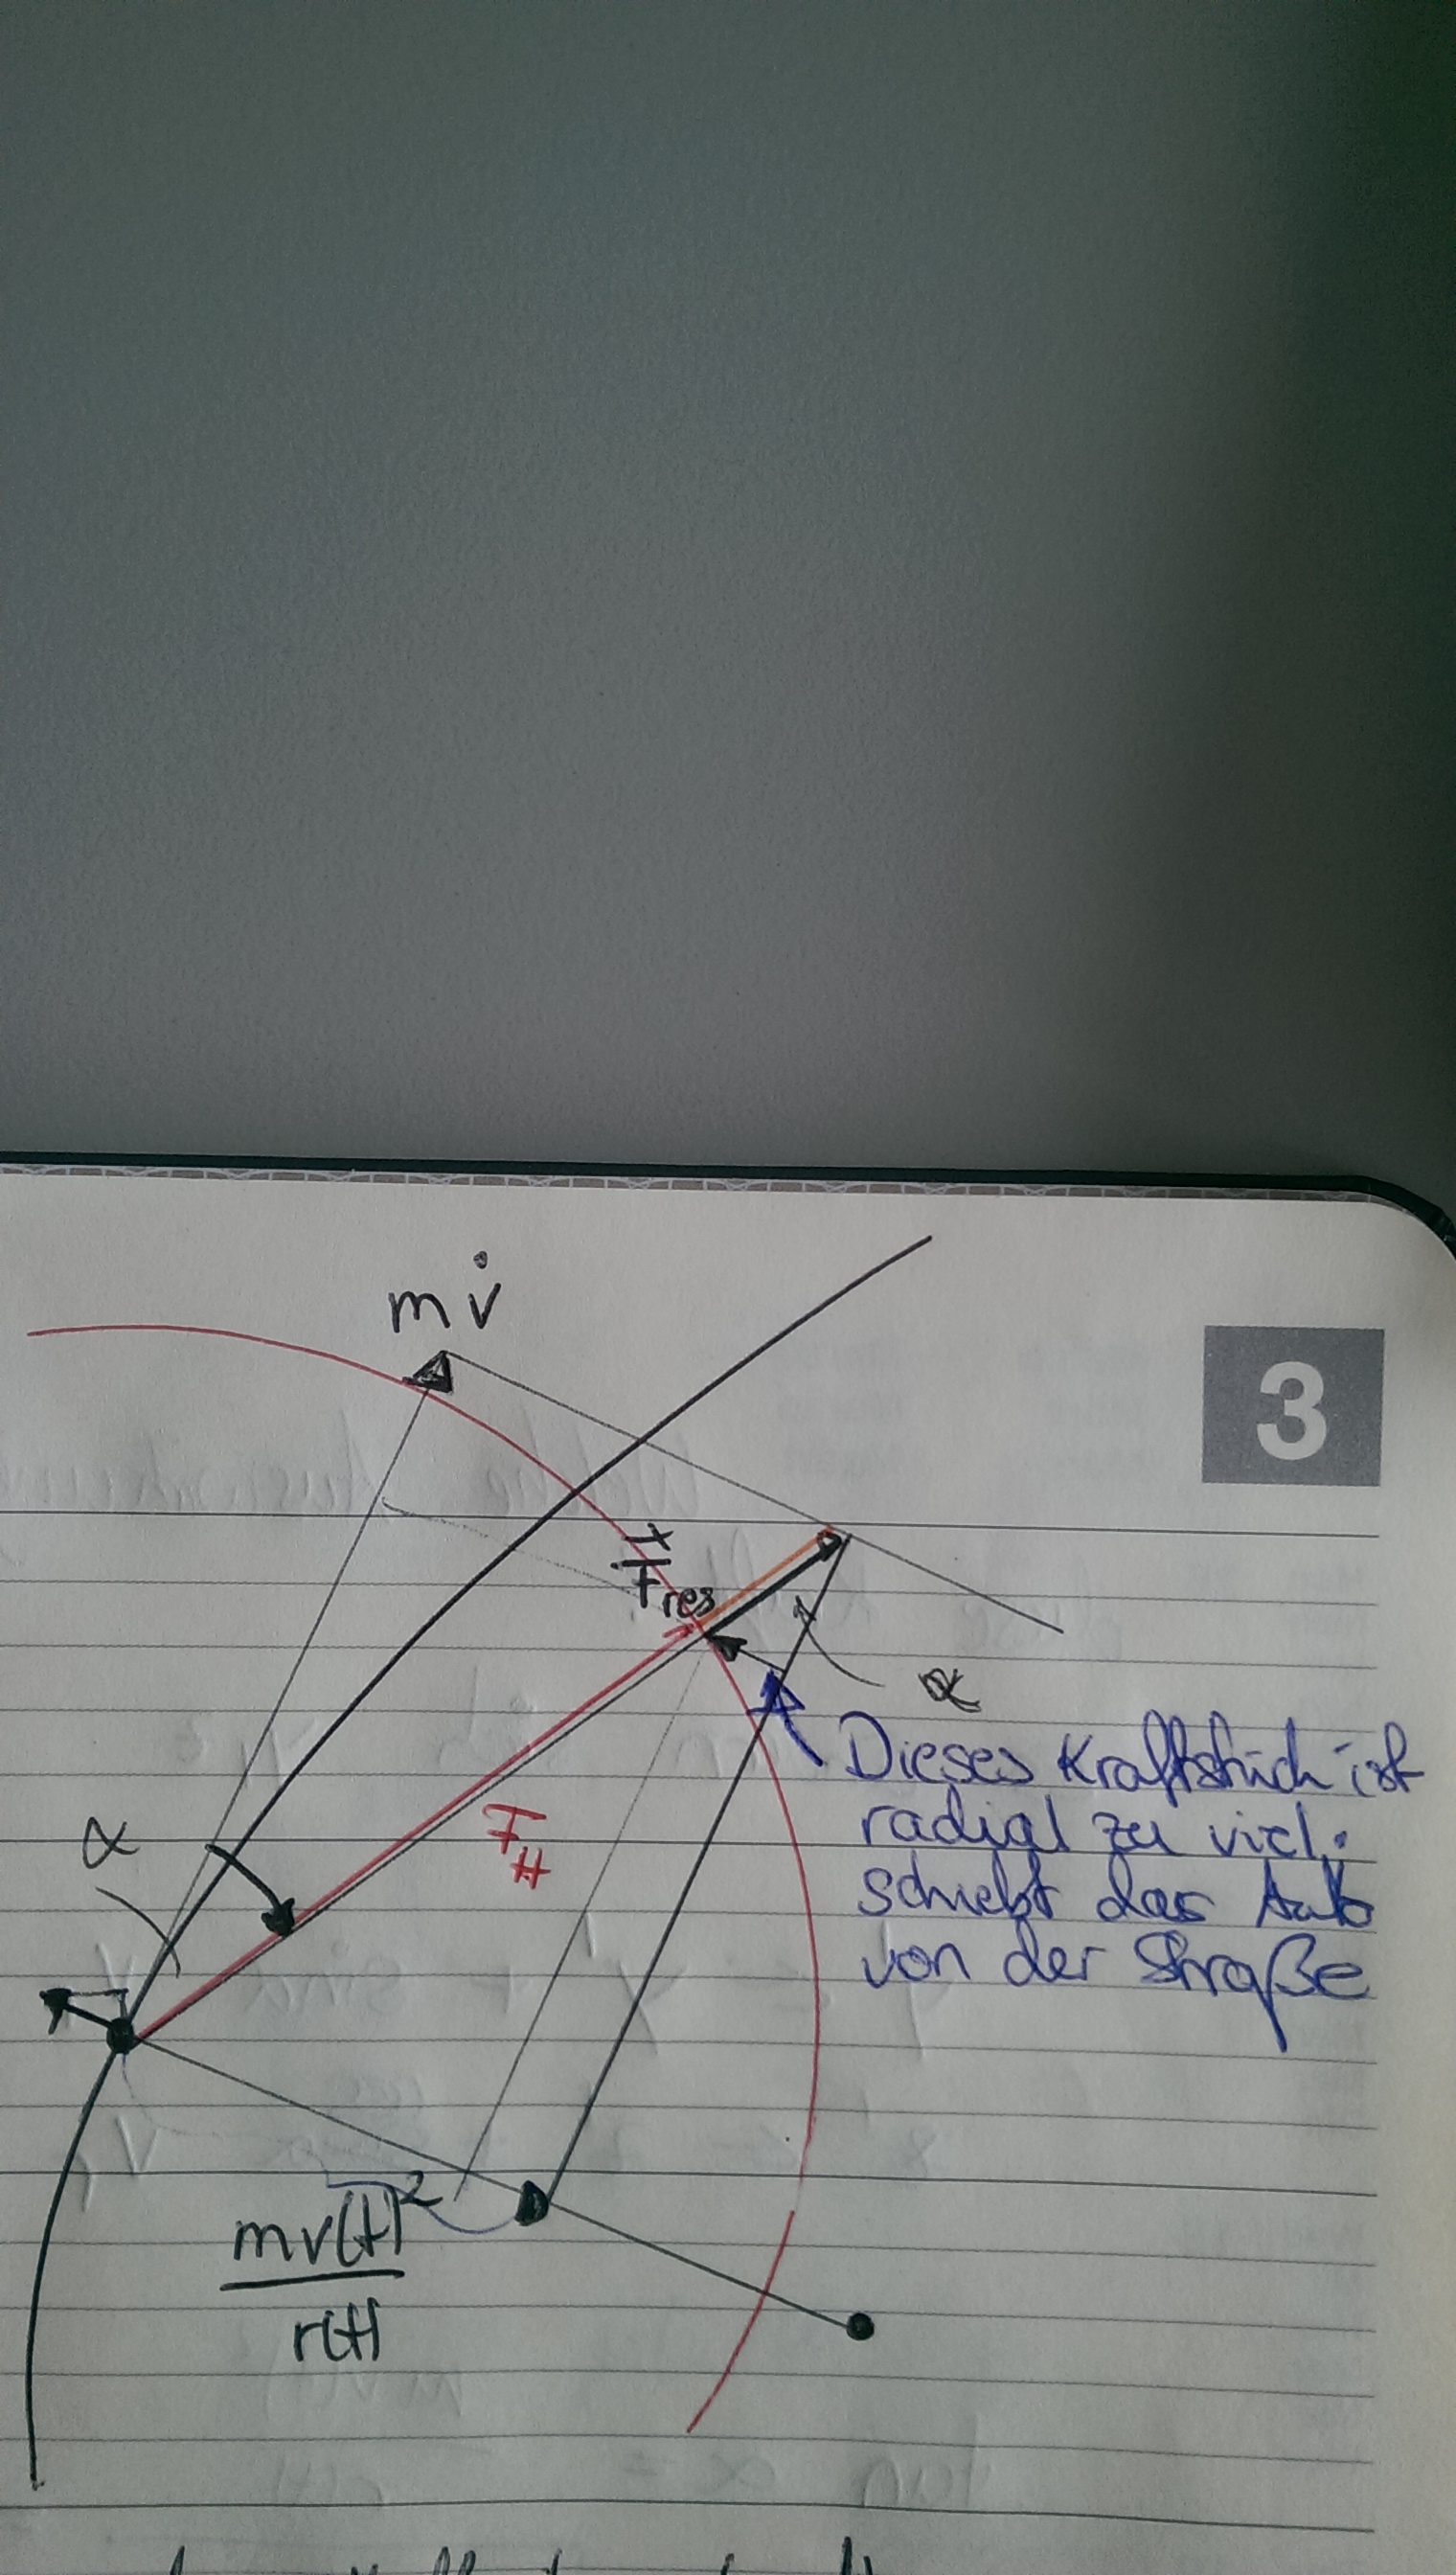
\includegraphics[angle = 270, scale=0.1]{pic}
\end{figure} 

\end{document}